\subsection{CONTINUITY AND DIFFERENTIABILITY OF CONVEX FUNCTIONS}

PROPOSITION 5. For a real finite function f to be convex (resp. strictly convex) on an interval I it is necessary and sufficient that for all \(a \in I\) the gradient

\[
p (\mathbf {M} _ {a} \mathbf {M} _ {x}) = \frac {f (x) - f (a)}{x - a}
\]

be an increasing (resp. strictly increasing) function of x on I ∩ ∁\{a\}.

This proposition is an immediate consequence of definitions 1 and 2 and of the lemma of I, p.~23.

PROPOSITION 6. Let \(f\) be a finite real function convex on an interval \(\mathbf{I} \subset \mathbf{R}\) . Then at every interior point \(a\) of \(\mathbf{I}\) the function \(f\) is continuous, has finite right and left derivatives, and \(f_g'(a) \leqslant f_d'(a)\) .

Indeed, for \(x \in I\) and \(x > a\) the function \(x \mapsto \frac{f(x) - f(a)}{x - a}\) is increasing (prop. 5) and bounded below, since if \(y < a\) and \(y \in I\) we have

\[
\frac {f (y) - f (a)}{y - a} \leqslant \frac {f (x) - f (a)}{x - a}\tag{5}
\]

by prop. 5; this function therefore has a finite right limit at the point \(a\) ; in other words, \(f_d'(a)\) exists and is finite; further, letting \(x\) approach \(a\) ( \(x > a\) ) in (5), it follows that

\[
\frac {f (y) - f (a)}{y - a} \leqslant f _ {d} ^ {\prime} (a)\tag{6}
\]

for all \(y < a\) belonging to I. In the same way one shows that \(f_{g}^{\prime}(a)\) exists and that

\[
f _ {d} ^ {\prime} (a) \leqslant \frac {f (x) - f (a)}{x - a}\tag{7}
\]

for \(x \in I\) and x \textgreater{} a. On letting x approach \(a (x > a)\) in this last inequality we obtain \(f_{g}^{\prime}(a) \leqslant f_{d}^{\prime}(a)\) . The existence of the left and right derivatives at the point a clearly ensures the continuity of f at this point.

COROLLARY 1. Let \(f\) be a convex (resp. strictly convex) function on I; if \(a\) and \(b\) are two interior points of I such that \(a < b\) one has (fig.~3)

\pandocbounded{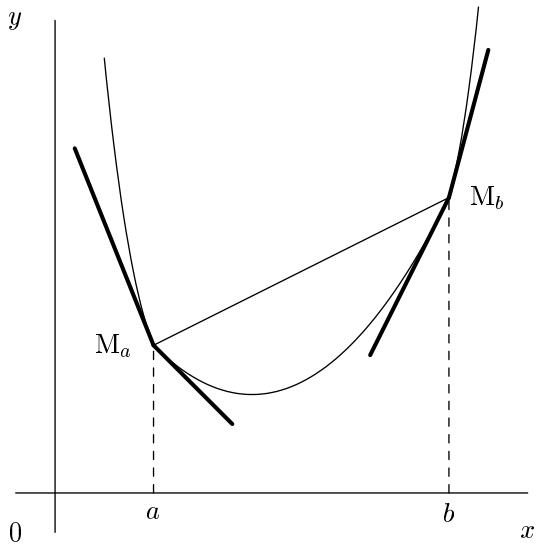
\includegraphics[keepaspectratio]{images/part001_a227d9e4.jpg}}\\
Fig. 3

\[
f _ {d} ^ {\prime} (a) \leqslant \frac {f (b) - f (a)}{b - a} \leqslant f _ {g} ^ {\prime} (b)\tag{8}
\]

(resp.

\[
f _ {d} ^ {\prime} (a) <   \frac {f (b) - f (a)}{b - a} <   f _ {g} ^ {\prime} (b)).\tag{9}
\]

The double inequality (8) results from (6) and (7) by a simple change of notation. On the other hand, if \(f\) is strictly convex and \(c\) is such that \(a < c < b\) one has, from (8) and prop. 5,

\[
f _ {d} ^ {\prime} (a) \leqslant \frac {f (c) - f (a)}{c - a} <   \frac {f (b) - f (a)}{b - a} <   \frac {f (b) - f (c)}{b - c} \leqslant f _ {g} ^ {\prime} (b)
\]

from which (9).

COROLLARY 2. If f is convex (resp. strictly convex) on I then \(f_{d}^{\prime}\) and \(f_{g}^{\prime}\) are increasing (resp. strictly increasing) on the interior of I; the set of points in I at which f is not differentiable is countable, and \(f_{d}^{\prime}\) and \(f_{g}^{\prime}\) are continuous at every point where f is differentiable.

The first part follows immediately from (8) (resp. (9)) and the inequality

\[
f _ {g} ^ {\prime} (a) \leqslant f _ {d} ^ {\prime} (a).
\]

On the other hand, let E be the set of interior points x of I where f is not differentiable (that is \(f_{g}^{\prime}(x) < f_{d}^{\prime}(x)\) ). For each \(x \in E\) let \(J_{x}\) be the open interval \(]f_{g}^{\prime}(x), f_{d}^{\prime}(x)[;\) it follows from (8) that if x and y are two points of E such that x \textless{} y, then u \textless{} v for all \(u \in J_{x}\) and all \(v \in J_{y}\) ; in other words, as x runs through E the open nonempty intervals \(J_{x}\) are pairwise disjoint; the set of such intervals is thus countable, and hence so is E. Finally, \(f_{d}^{\prime}\) (resp. \(f_{g}^{\prime}\) ) being increasing, it has a right limit and a left limit at every interior point x of I; prop. 6 of I, p.~18 now shows that the right limit of \(f_{d}^{\prime}\) (resp. \(f_{g}^{\prime}\) ) at the point x is equal to \(f_{d}^{\prime}(x)\) , and its left limit is \(f_{g}^{\prime}(x)\) ; from which we have the last part of the corollary.

Let \(f\) be a convex function on \(I, a\) an interior point of \(I\) , and \(D\) a line passing through the point \(M_a\) , with equation \(y - f(a) = \alpha(x - a)\) . It follows from the inequalities (8) that if \(f_g'(a) \leqslant \alpha \leqslant f_d'(a)\) then every point of the graph \(G\) lies above \(D\) , and, if \(f\) is strictly convex, \(M_a\) is the only point common to \(D\) and \(G\) ; one says that \(D\) is a support line to \(G\) at the point \(M_a\) . Conversely, if \(G\) lies above \(D\) , one has \(f(x) - f(a) \geqslant \alpha(x - a)\) for every \(x \in I\) , from which \(\frac{f(x) - f(a)}{x - a} \geqslant \alpha\) for \(x > a\) , and \(\frac{f(x) - f(a)}{x - a} \leqslant \alpha\) for \(x < a\) ; on letting \(x\) tend to \(a\) in these inequalities it follows that \(f_g'(a) \leqslant \alpha \leqslant f_d'(a)\) .

In particular, if \(f\) is differentiable at the point \(a\) there is only one supporting line to \(G\) at the point \(M_a\) , the tangent to \(G\) at \(M_a\) .

Remark. If \(f\) is a strictly convex function on an open interval \(I\) then \(f_d'\) is strictly increasing on \(I\) , so there are three possible cases, according to prop. 2 of \(I\) , p.~13:

\(1^{\circ} f\) is strictly decreasing on I;

\(2^{\circ}\) f is strictly increasing on I;

\(3^{\circ}\) there is an \(a \in \mathrm{I}\) such that \(f\) is strictly decreasing for \(x \leqslant a\) , and is strictly increasing for \(x \geqslant a\) .

When \(f\) is convex on \(I\) , but not strictly convex, \(f\) can be constant on an interval contained in \(I\) ; let \(J = ]a, b[\) be the largest open interval on which \(f\) is constant (that is to say, the interior of the interval where \(f_{d}^{\prime}(x)=0\)) ; then f is strictly decreasing on the interval formed by the points \(x\in I\) such that \(x\leqslant a\) (if it exists), strictly increasing on the interval formed by the points \(x\in I\) such that \(x\geqslant b\) (if it exists).

In all cases one sees that \(f\) possesses a right limit at the left-hand endpoint of I (in \(\overline{\mathbf{R}}\) ), and a left limit at the right-hand endpoint; these limits may be finite or infinite (cf.~I, p.~46, exerc. 5, 6 and 7). By abuse of language one sometimes says that the continuous function (with values in \(\overline{\mathbf{R}}\) ), equal to \(f\) on the interior of I, and extended by continuity to the endpoints of I, is convex on \(\overline{\mathbf{I}}\) .

